\section{Simulation Experiments and Results}
\label{sec:experiments}

The simulation code is supplied with the paper \cite{code_active_inference_2026} so that readers can reproduce the experiments, vary the conditions, and inspect the resulting localization behavior directly.

This section is organized as a progression toward a real-robot test environment. This is evaluated in two complementary ways. First, convergence scenarios use many randomized trials to test whether the belief can recover from different initial field positions and reach centimeter-level localization without landmark ambiguity. Next, tracking scenarios test whether the belief remains stable over time while the robot moves under noise, dropout, limited field of view, obstruction, and landmark ambiguity.

\begin{figure}[t]
    \centering
    \begin{minipage}[t]{0.55\linewidth}
        \vspace{0pt}
        \centering
        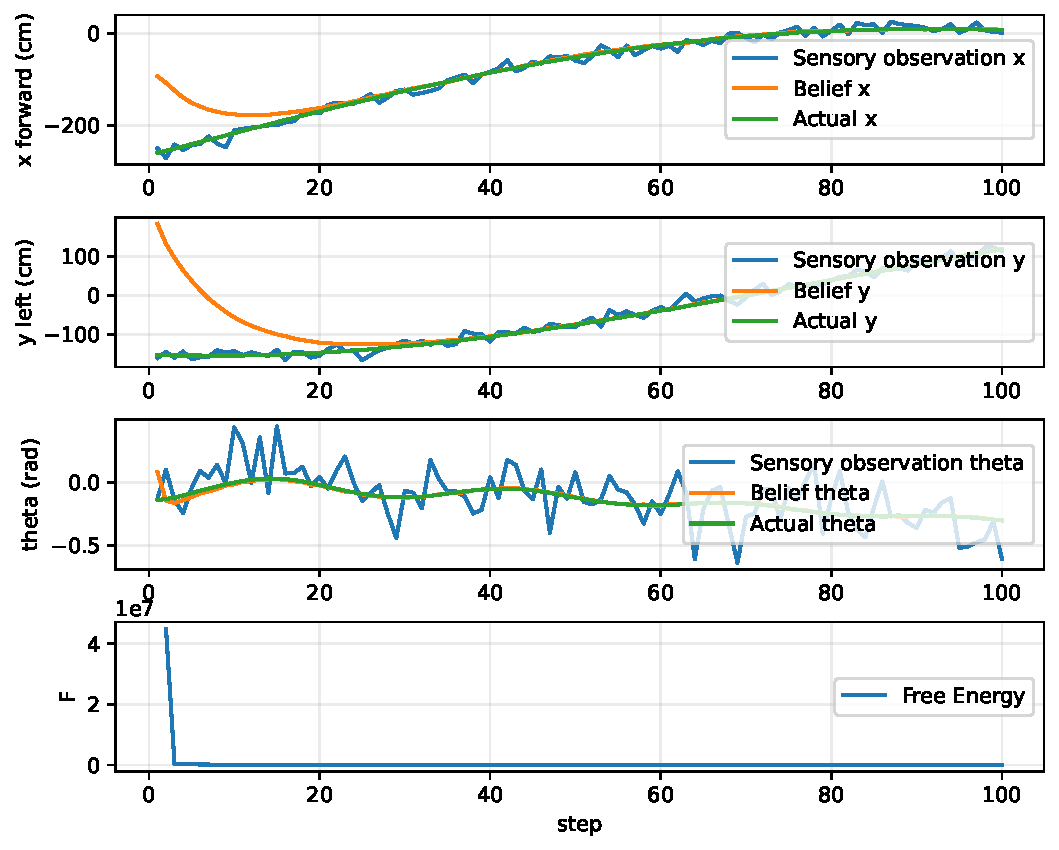
\includegraphics[width=0.95\linewidth,page=1]{figures/paper_experiment_20260611_141048.pdf}\\
        \small (a) Position and orientation tracking
    \end{minipage}
    \hfill
    \begin{minipage}[t]{0.42\linewidth}
        \vspace{0pt}
        \centering
        \includegraphics[width=0.95\linewidth,page=2]{figures/paper_experiment_20260611_141048.pdf}\\
        \small (b) Velocity components

        \vspace{0.25em}

        \includegraphics[width=0.95\linewidth,page=3]{figures/paper_experiment_20260611_141048.pdf}\\
        \small (c) Acceleration components
    \end{minipage}
    \caption{\scriptsize Representative moving-robot belief estimate with 9 landmarks, 10 cm landmark noise, $10^\circ$ angular noise, and 10\% motion noise. Starting from a random belief and random actual pose, the belief starts tracking the actual pose. The actual robot follows a "circle" path. The velocity and acceleration plots show that the update estimates generalized-coordinate dynamics rather than only a pose estimate.}
    \label{fig:typical-experiment-results}
\end{figure}
\FloatBarrier

\subsection{Static Robot Scenarios}
\label{subsec:experiments-static}

The method is first tested in the most basic static scenario: the robot is not moving, and its position must be determined from unambiguous landmark observations.
Table~\ref{tab:static-convergence-results} shows 100\% convergence across all tested static scenarios. The landmark update can recover the correct field pose from randomized start positions, even when only a limited number of visible landmarks is available. In the near-start condition with 9 visible landmarks, convergence required only $23.6 \pm 5.0$ inference steps. Fewer available landmarks, noise or obstruction increased the number of inference steps needed for convergence.

\begin{table}[!htbp]
    \centering
    \caption{\scriptsize Static robot convergence results with unique-ID data association. A trial is counted as successful when the belief reaches the actual pose within 3 cm position error and 3 degrees orientation error for at least five consecutive inference steps. Random means that the actual pose and the initial belief pose are sampled independently from random field positions, covering captured-robot-style recovery from an arbitrary wrong pose. Near means that the belief pose is sampled near the actual pose, offset by at most 50 cm in $x/y$ and 20 degrees in heading. Noise reports the shared landmark-position noise in centimeters, landmark-angle noise in degrees, and motion noise in percent.}
    \label{tab:static-convergence-results}
    \scriptsize
    \begin{tabular}{rrrrrlllll}
        \toprule
        N & Success & Mean & SD & P99 & Start & LM & Hz & Noise & Drop \\
        \midrule
        1000 & 100\% & 55.8 & 19.1 & 132 & Random & 9 & 40 & None & None \\
        1000 & 100\% & 23.6 & 5.0 & 36 & Near & 9 & 40 & None & None \\
        1000 & 100\% & 45.9 & 14.4 & 101 & Random & 9 & 200 & None & None \\
        1000 & 100\% & 63.9 & 22.1 & 149 & Random & 9 & 40 & 10 & 10\% \\
        1000 & 100\% & 129.4 & 85.3 & 467 & Random & 5 & 40 & None & None \\
        1000 & 100\% & 259.8 & 105.4 & 609 & Random & 2 & 40 & None & None \\
        1000 & 100\% & 48.2 & 20.4 & 113 & Near & 5 & 40 & 10 & 10\% \\
        1000 & 100\% & 112.0 & 40.7 & 225 & Near & 2 & 40 & 10 & 10\% \\
        \bottomrule
    \end{tabular}
\end{table}
\FloatBarrier

\subsection{Dynamic Robot Scenarios}
\label{subsec:experiments-dynamic}

The next question is whether the algorithm can converge while the actual robot is moving. Table~\ref{tab:dynamic-convergence-results} shows 100\% convergence across all tested dynamic scenarios. In the near-start condition with 9 visible landmarks, convergence required only $44.2 \pm 22.4$ inference steps. The moving-robot results follow the same main trend as the static tests: fewer available landmarks, noise and obstruction increase the number of inference steps needed for convergence, but do not prevent recovery in these tests with unambiguous landmarks.

The representative noisy run in Fig.~\ref{fig:typical-experiment-results} illustrates this behavior. The belief starts away from the actual pose, is corrected by motion and landmark prediction errors, and then remains close to the moving actual robot. The velocity and acceleration plots show that the update estimates a generalized-coordinate belief rather than only a static pose.

\begin{table}[!htbp]
    \centering
    \caption{\scriptsize Dynamic robot convergence results. The actual robot follows a Random targets path with speeds up to 5 m/s and accelerations up to 12 m/s$^2$. Tests follow the same definitions as Table~\ref{tab:static-convergence-results}.}
    \label{tab:dynamic-convergence-results}
    \scriptsize
    \begin{tabular}{rrrrrlllll}
        \toprule
        N & Success & Mean & SD & P99 & Start & LM & Hz & Noise & Drop \\
        \midrule
        1000 & 100\% & 61.4 & 19.0 & 119 & Random & 9 & 40 & None & None \\
        1000 & 100\% & 44.2 & 22.4 & 105 & Near & 9 & 40 & None & None \\
        1000 & 100\% & 53.5 & 22.8 & 140 & Random & 9 & 200 & None & None \\
        1000 & 100\% & 74.9 & 28.2 & 163 & Random & 9 & 40 & 10 & 10\% \\
        1000 & 100\% & 121.2 & 57.4 & 308 & Random & 5 & 40 & None & None \\
        1000 & 100\% & 388.5 & 248.8 & 1313 & Random & 2 & 40 & None & None \\
        1000 & 100\% & 93.6 & 60.5 & 267 & Near & 5 & 40 & 10 & 10\% \\
        1000 & 100\% & 289.4 & 234.6 & 1157 & Near & 2 & 40 & 10 & 10\% \\
        \bottomrule
    \end{tabular}
\end{table}
\FloatBarrier

\subsection{Tracking Duration Test}
\label{subsec:experiments-visibility-stress}

Tracking duration tests shift the focus from convergence to sustained tracking under partial and interrupted landmark visibility. To approximate humanoid robot-soccer perception, landmark visibility is restricted to a representative 110-degree field of view, and the simulation includes 2-second obstruction periods in which other robots temporarily block relevant field landmarks.

Under the combined conditions of noise, dropout, limited field of view, and temporary obstruction, the method remained stable over a 2-hour Random targets run initialized from a near-start belief. The result is not error-free tracking at every instant, but stable recovery: motion terms keep the belief evolving during weak landmark evidence, and later landmark observations correct accumulated deviations. Table~\ref{tab:visibility-stress-tracking-summary} summarizes this behavior. The left panel reports post-settling component-error bands; the right panel shows recovery with multiple landmarks.

\begin{table}[!htbp]
    \centering
    \caption{\scriptsize Moving visibility-stress tracking summary over a 2-hour near-start Random targets run with unique-ID landmark association, 40 Hz profile, noise, dropout, 110-degree field of view, and temporary obstruction enabled. Left: percentage of post-settling timesteps at or below each component-error band. While moving the robot heading keeps rotating toward (300 cm, 0 cm). Right: median future-minus-current change in absolute component error over the next 2 seconds, grouped by the number of visible landmarks; negative values indicate correction toward the actual pose.}
    \label{tab:visibility-stress-tracking-summary}
    \scriptsize
    \begin{minipage}[t]{0.49\linewidth}
        \centering
        \textbf{(a) Tracking precision}\\[0.25em]
        \setlength{\tabcolsep}{5pt}
        \begin{tabular}{lccc}
            \toprule
            Band & $|x|$ & $|y|$ & $|\theta|$ \\
            \midrule
            3 cm / 3 deg & 35.09\% & 28.60\% & 99.74\% \\
            5 cm / 5 deg & 55.24\% & 46.57\% & 99.99\% \\
            7.5 cm / 7.5 deg & 73.98\% & 65.32\% & 100.00\% \\
            10 cm / 10 deg & 86.06\% & 79.07\% & 100.00\% \\
            15 cm / 15 deg & 96.82\% & 93.67\% & 100.00\% \\
            20 cm / 20 deg & 99.35\% & 98.32\% & 100.00\% \\
            25 cm / 25 deg & 99.91\% & 99.57\% & 100.00\% \\
            30 cm / 30 deg & 99.98\% & 99.89\% & 100.00\% \\
            \bottomrule
        \end{tabular}
    \end{minipage}
    \hfill
    \begin{minipage}[t]{0.49\linewidth}
        \centering
        \textbf{(b) Two-second error change}\\[0.25em]
        \setlength{\tabcolsep}{4pt}
        \begin{tabular}{lrrrr}
            \toprule
            LM & N & $\Delta |x|$ & $\Delta |y|$ & $\Delta |\theta|$ \\
            \midrule
            0--1 & 5294 & +0.87 cm & +2.57 cm & -0.15 deg \\
            2--3 & 70406 & +0.18 cm & +1.39 cm & -0.01 deg \\
            4--5 & 151561 & -0.11 cm & -0.19 cm & -0.00 deg \\
            6+ & 60260 & -0.09 cm & -1.16 cm & -0.00 deg \\
            \bottomrule
        \end{tabular}
    \end{minipage}
\end{table}

\FloatBarrier

\subsection{Tracking Duration Test Under Landmark Ambiguity}
\label{subsec:experiments-landmark-ambiguity}

The next stress condition tests landmark ambiguity. Many soccer-field landmarks are geometrically repeated, so a local observation does not always identify a unique field location. For example, an observed field corner can correspond to any of the four physical field corners. This creates a data-association problem: the algorithm must decide which known FCS landmark generated the RCS observation before the prediction error can be used for belief updating.

In this proof of concept, ambiguity is handled with gated nearest-neighbor association. For each observed landmark type, candidate map landmarks of the same type are projected into RCS from the current belief; the closest candidate is selected only if its prediction error falls within a gating threshold. Otherwise, the observation is rejected for that update step. This is a deliberately simple and pragmatic association strategy. Although more advanced multi-hypothesis approaches were considered, the simulations showed that gated nearest-neighbor matching was sufficient for the present proof of concept. With landmark ambiguity enabled, the method maintained stable tracking when initialized from a converged belief.


\begin{table}[!htbp]
    \centering
    \caption{\scriptsize Tracking with landmark ambiguity, under the same conditions as Table~\ref{tab:visibility-stress-tracking-summary}}
    \label{tab:landmark-ambiguity-tracking}
    \scriptsize
    \setlength{\tabcolsep}{5pt}
    \begin{tabular}{lccc}
        \toprule
        Band & $|x|$ & $|y|$ & $|\theta|$ \\
        \midrule
        3 cm / 3 deg & 34.76\% & 28.58\% & 99.73\% \\
        5 cm / 5 deg & 54.58\% & 46.00\% & 99.98\% \\
        7.5 cm / 7.5 deg & 73.44\% & 64.61\% & 100.00\% \\
        10 cm / 10 deg & 85.66\% & 78.30\% & 100.00\% \\
        15 cm / 15 deg & 96.65\% & 93.32\% & 100.00\% \\
        20 cm / 20 deg & 99.31\% & 98.13\% & 100.00\% \\
        25 cm / 25 deg & 99.88\% & 99.54\% & 100.00\% \\
        30 cm / 30 deg & 99.99\% & 99.87\% & 100.00\% \\
        \bottomrule
    \end{tabular}
\end{table}
\FloatBarrier
